%!TEX root = ../main.tex

\section{Modelling Data}
The modelling of data in this thesis is the vital first step to the optimization of a dragline, any simplifications made in this step will carry through all steps of the algorithm and effect the accuracy of the final results, therefore the manipulation of data to suit the system must be considered very carefully. As the dimensionality of the data decreases the runtime will as well, however the achievable accuracy will decrease as the system will become more general. The method selected for the modelling of the geological data is a one dimensional density function used to represent the amount of overburden required to be removed from the mine along a specific strip. 
% While this is not ideal in terms of a truly optimal solution it will allow the program to run rapidly, many assumptions along the way will result in loss of optimality at many stages, while an optimal solution is the desired result any feasible or near optimal solution is also acceptable. 
While simplifications could cause discrepancies between real world performance and the results suggested by the model, while this is not ideal the simplifications should reduce the time taken for calculation. The trade off between accuracy and time taken to calculate results is a difficult one to make, however is made easier by the fact that methods exist for the calculation of a block in 3D \cite{ORLeslie}and if the simplifications are too unrealistic then these models could be substituted in. 
\\


An alternate approach that was considered was the use of machine learning or metahueristics, however these methods would require huge amounts of data \cite{Meta} which was not readily available during this thesis. These approaches should be considered  to calculate either the optimisation of strip or block as they would result in potentially accurate and useful models, however the lack of data made such approaches infeasible.

One dimensional density functions are also useful as they can be generated through two methods, either through a generated data set for testing or through geological survey data. In the thesis the sample data was generated by generating typical mine shapes and layouts of interest, such as a ramp and step function; within these samples a noise function was applied to give a better and more realistic set of data to test on samples of these mines can be seen below in figures \ref{Minestep} \& \ref{MineRand}. 
\\
Survey data was supplied in a .xyz format, by assuming a constant depth of cut and a homogeneous packing density of overburden,the average depth along the width for each one metre section was taken for the length of the strip. This data represents the average amount of overburden present at each section of the mine.  This  data was represented as an array for ease of use in python, an additional reason for this decision is that the mine will always be mined in order \cite{MiningHandbook} and as such the list will simply be traversed from start to end.  

\begin{figure}[h]
\caption{A Generated mine (Step Function)}
\label{Minestep}
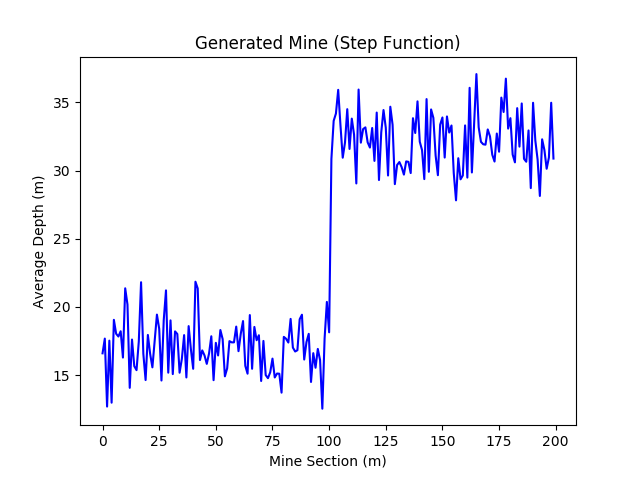
\includegraphics[width=\textwidth]{StepMine.png}
\end{figure}
\begin{figure}[h]
\caption{A Generated mine (Random Function)}
\label{MineRand}
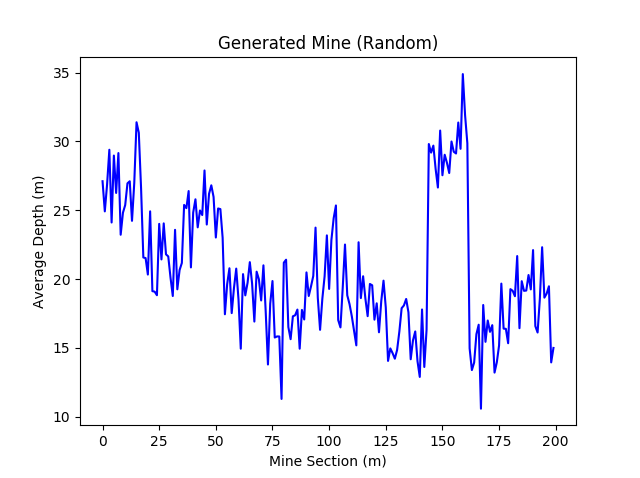
\includegraphics[width=\textwidth]{RandMine.png}
\end{figure}




\subsection{Types of Input}
The intended use of the program is to rapidly calculate optimal, near optimal or feasible block dimensions for a single strip inside a mine.  The implementation of this would allow on the fly adjustments and the ability to make corrections and compensations for errors. The adjustment and use of the program for an end user is out of the scope of this project as the thesis focuses more on the algorithms and underlying principles of the software rather than the user interface and user experience. Rather it should be assumed that the inputs to the project are a 1 dimensional array representing the spoil and another representing the overburden. The program can have the specifics of the dragline altered so that other applicable machines can be considered, while this is simple to change there is no user interface for the program and as such if it were to see further use then a graphic user interface would need to be constructed. \\


\section{Cost of Overburden Movement}
% The cost of a block is vital to the solution to the problem, however the cost of a block is calculated as a summation of many individual movements, therefore the proper consideration for these models should be undertaken, ideally the cost of overburden movement will be able to calculate the time of movement for the action of moving overburden from point $n$ in the mine to $s$ in the spoil strip. Therefore two inputs would be the only required information for this function.
The cost of a block is required when calculating the cost of an overall strip as well as when considering blocks of differing sizes. The model is required to calculate the cost of movement when removing overburden from a mine and depositing it into the spoil channel. This function will be predominantly inspired by the work mentioned in section 3.1 as these validations are not able to be reproduced with the limited data available. 
\subsection{Scope}
The function to calculate the cost of an action is required to work for all $n\in N , s \in S$ if this movement is at all valid, therefore we can assume that only valid entries will be passed into this solution. Therefore for any valid combination the function should return a cost of movement, while the cost function is not required to be linear it must be able to be used in a linear programming engine such as Gurboi \cite{gurobi}, and as such must be linearly related to block usage for objective functions. This is the most pressing constraint as otherwise linear programming will be unable to be used.
\subsection{Assumptions}
The assumption made in this section is that the function can calculate a reasonable model of the cost of movement through a continuous function of one input. This formulation takes the cost of movement within a block to be the time taken to move material, dragline movement is ignored as it will be similar for any length of block \cite{Costs}. Other costs associated with overburden removal are not considered in this formulation as the implementation of such would require additional information into the specific digging pattern the dragline is performing.
% \subsection{Justification}

\section{Cost of a Block}
A cost model of a block is required to cost the excavation of an entire strip within a  mine,  each block will have a cost dependant on its location within the mine, its size and the state of the spoil prior to excavating the block. The function must be able to be calculated quickly as it will be called many times. Two  formulations were considered for this element of the problem, Linear programming and dynamic programming methods were attempted both inspired by the work outlined in section 3.2.
\subsection{Assumptions}
The assumptions are as follows: \begin{itemize}
\item The cost of movement through a block can be ignored.
\item The swing time is be representative of the cost of the block.
\item The cost of a block is able to be calculated in a reasonably accurate in a one dimensional environment.
\item The block is mined sequentially with no consideration to the specific movement pattern of the mine.
\item All overburden will be removed from the current section before the next section is considered.
\item The reach of the dragline will be considered from the location of the current block. 
 \end{itemize}

\subsection{Justification}
The modelling of a block in this simplistic method is valid as the most important attribute with the block model is that the results are analogous to other models.  However the model selected is a reasonable approximation of overburden removal for each block as is should represent the most basic of dragline movement patterns throughout the block. This is further reinforced in  section 6.1 where the models applied in this thesis are compared against an industry validated model \cite{ORLeslie}.More complex patterns require that the model is updated, however typically more complex models will require a higher dimensionality of data and therefore this model would have to be reconsidered.  


\section{Cost of a Strip}
The cost of a strip must be calculated in a way such that the cost of all total blocks is considered and minimised, the cost of blocks as well as a constant for starting a new block is the only cost associated with the cost of a strip. This assumption means that the cost of a strip is independent on all other actions that precede it but that the spoil is updated as the strip is mined, furthermore the length of the strip must be defined before the mining has begun such that the desired strip length is already defined as the allowable length of the mine. 
\subsection{Assumptions} 
The strip must be removed entirely and the length of the strip cannot be increased as this may be unallowable and cannot be decreased as the savings in time are offset by the loss of potential profit, furthermore it is assumed that there is some additional cost in time for the starting of a new block associated with the set up of machinery and relocation of equipment. 
\subsection{Justification}
The suggested model is a valid application of ordering of blocks in a way to reduce the cost of actions independently of the block model, this means that if the block model is changed the method of optimising the strip will remain the same, this independence of both models allows changes and improvements to be made without interfering with the other parts of the formulation. 

% \section{Communication of Results}
% \subsection{Scope}
% \subsection{Assumptions}
% \subsection{Demonstration}